\chapter{Практическая часть}
\section{Построение примеров вычислений и использования}
Рассмотрим систему уравнений (5) и её решение $ P_0, Q_0 $
$$ A \Phi(A_S^T P_0, -A_F^T P_0) = Q_0 $$
А также перенумерованные векторы $ P_0 $ и $ Q_0 $ так, чтобы сначала шли узлы с заданными притоками, затем с давлениями

$$ P_0 = \left(\frac{P_0^{var}}{P_0^{fix}}\right), Q_0 = \left(\frac{Q_0^{var}}{Q_0^{fix}}\right) $$
и их "малые" изменения

$$ \delta P_0 = \left(\frac{ \delta P_0^{var}}{ \delta P_0^{fix}}\right), \delta Q_0 = \left(\frac{ \delta Q_0^{var}}{ \delta  Q_0^{fix}}\right) $$

В соотстветствие с описанным выше способом, получается:

$$ dQ_0^{var} = [ M_{PQ} M^{-1} ] ( A_S^T P_0, -A_F^T P_0  ) dQ_0^{fix} + $$ $$ [ M_{PP} - M_{PQ} M^{-1} M_{QP} ] ( A_S^T P_0, -A_F^T P_0 ) dP_0^{fix} $$

Соответственно вектор откликов притоков

$$ dP_0^{var} = [M^{-1}](A_S^T P_0, -A_F^T P_0) dQ_0^{fix} - [M^{-1} M_{QP}](A_S^T P_0, -A_F^T P_0) dP_0^{fix} $$

и вектор откликов давлений.
\section{Примеры вычислений}

Все примеры носят иллюстративный характер.

\subsection{Пример 1}

\begin{figure}[h]
  \center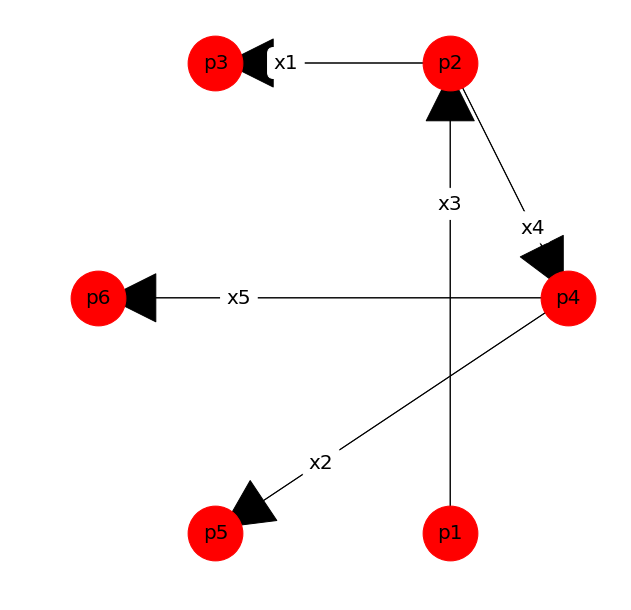
\includegraphics[width=0.6\linewidth]{picts/example1/1.png}
  \caption{Схема для примера 1}
  \label{fig:example_1}
\end{figure}

Рассмотрим простую гидравлическую цепь, изображенную на рисунке 3.1.

На данной схеме в узлах графа задаются давления, на рёбрах расходы.

\begin{table}[h!]
  \centering
    \begin{tabular}{| l | c |}
    \hline
    Переменная & Значение \\ \hline
    $ P_1 $ & 18 \\ \hline
    $ P_3 $ & 4 \\ \hline
    $ P_5 $ & 7 \\ \hline
    $ P_6 $ & 6 \\ \hline

    \end{tabular}
  \caption{Начальные условия}
\end{table}

Начальные условия представлены в таблице 3.1. Также, их можно отобразить на рисунке.

\begin{figure}[h]
  \center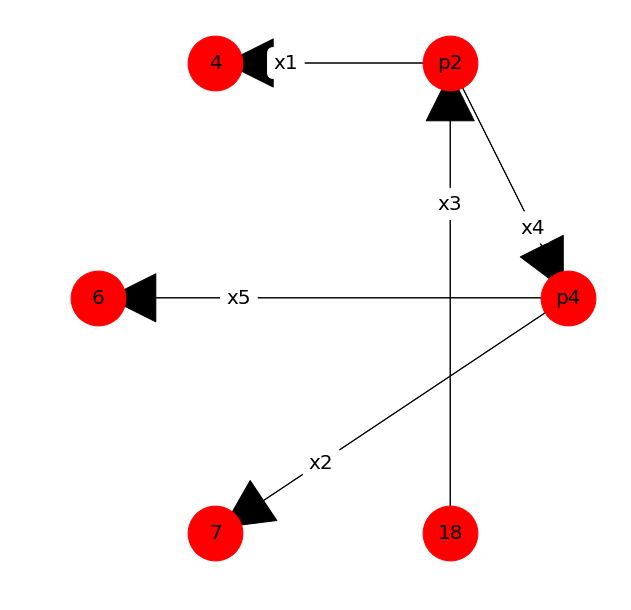
\includegraphics[width=0.7\linewidth]{picts/example1/2.png}
  \caption{Схема для примера 1 (с учетом начальных условий)}
  \label{fig:example_1}
\end{figure}

Далее по расчетной схеме получается система уравнений для решения задачи.

\[ 
\begin{cases} 
	P_4^2 - P_6^2 - A X_5^2 = 0 \\
	P_4^2 - P_5^2 - A X_2^2 = 0 \\
	P_2^2 - P_4^2 - A X_4^2 = 0 \\
	P_2^2 - P_3^2 - A X_1^2 = 0 \\
	P_4^2 - P_6^2 - A X_5^2 = 0 \\
	P_1^2 - P_2^2 - A X_3^2 = 0 \\
	X_3 - X_1 - X_4 = 0 \\
	X_4 - X_2 - X_5 = 0 \\
\end{cases}
\]

Численное решение системы, с учетом начальных условий из таблицы 3.1, даёт значение неизвестных

\begin{table}[h!]
  \centering
    \begin{tabular}{| l | c |}
    \hline
    Переменная & Значение \\ \hline
    $ P_1 $ & 18 \\ \hline
    $ P_2 $ & 9.689 \\ \hline
    $ P_3 $ & 4 \\ \hline
    $ P_4 $ & 7.322 \\ \hline
    $ P_5 $ & 7 \\ \hline
    $ P_6 $ & 6 \\ \hline
    $ X_1 $ & 8.825 \\ \hline
    $ X_2 $ & 15.17 \\ \hline
    $ X_3 $ & 6.345 \\ \hline
    $ X_4 $ & 4.197 \\ \hline
    $ X_5 $ & 2.148 \\ \hline

    \end{tabular}
  \caption{Результаты расчета}
\end{table}

В результате найдены значения всех неизвестных. 

\begin{figure}[h]
  \center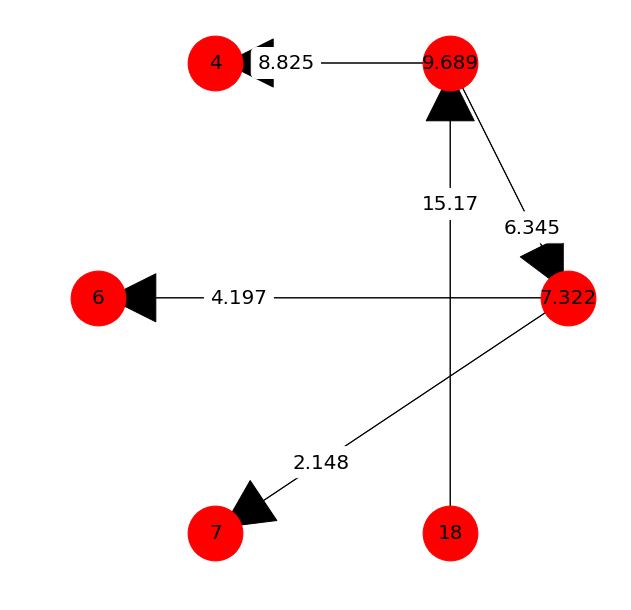
\includegraphics[width=0.7\linewidth]{picts/example1/3.png}
  \caption{Схема для примера 1 (все неизвестные учтены)}
  \label{fig:example_1}
\end{figure}

Теперь рассмотрим малое изменение начальных условий.

\begin{table}[h!]
  \centering
    \begin{tabular}{| c | c | c |}
    \hline
    Переменная & Предыдущее значение & Новое значение \\ \hline
    $ P_1 $ & 18 & 18.01 \\ \hline
    $ P_3 $ & 4 & 4.01 \\ \hline
    $ P_5 $ & 7 & 7.01 \\ \hline
    $ P_6 $ & 6 & 6.01 \\ \hline

    \end{tabular}
  \caption{Начальные условия (измененные)}
\end{table}

Новый расчет будет проведен 2-мя способами: будет решена система уравнений и с помощью матрицы чувствительности.

Результаты и сранение 2-х способов отображены в таблице 3.4.

\paragraph{Точное значение} -- получено из решения системы уравнений.

\paragraph{Оцененное значение} -- получено с помощью матрицы чувствительности.

\begin{table}[h!]
  \centering
    \begin{tabular}{| c | c | c |}
    \hline
    Переменная & Точное значение & Оцененное значение \\ \hline
    $ P_1 $ & 18.01 & 18.01 \\ \hline
    $ P_2 $ & 9.697 & 9.70 \\ \hline
    $ P_3 $ & 4.01 & 4.01 \\ \hline
    $ P_4 $ & 7.331 & 7.331 \\ \hline
    $ P_5 $ & 7.01 & 7.01 \\ \hline
    $ P_6 $ & 6.01 & 6.01 \\ \hline
    $ X_1 $ & 8.829 & 8.823 \\ \hline
    $ X_2 $ & 15.176 & 15.170 \\ \hline
    $ X_3 $ & 6.347 & 6.351 \\ \hline
    $ X_4 $ & 4.199 & 4.198 \\ \hline
    $ X_5 $ & 2.147 & 2.153 \\ \hline

    \end{tabular}
  \caption{Результаты расчета}
\end{table}

Из таблицы 3.4 видно, что разница между значениями переменных, полученными разными методами, весьма мала.

\subsection{Пример 2}
Аналогично, как и в примере 1, будут проведены расчеты разными методами и результаты будут отображены в таблице.

\begin{figure}[h]
  \center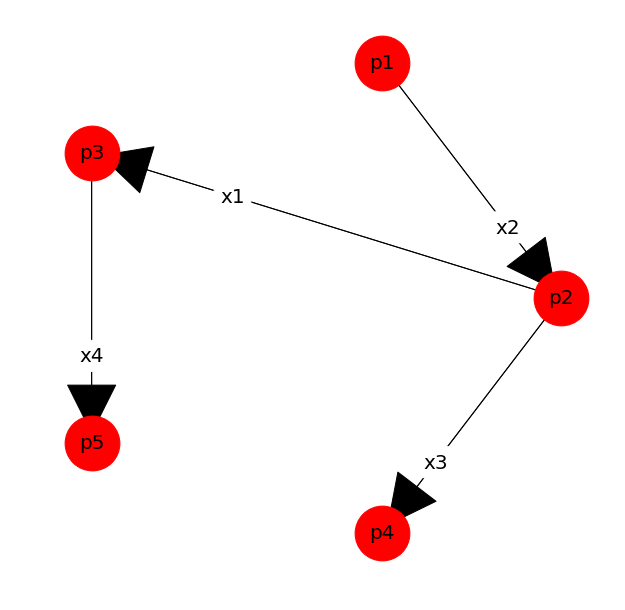
\includegraphics[width=0.7\linewidth]{picts/example2/1.png}
  \caption{Схема для примера 2}
  \label{fig:example_1}
\end{figure}


\begin{table}[h!]
  \centering
    \begin{tabular}{| l | c |}
    \hline
    Переменная & Значение \\ \hline
    $ P_1 $ & 10 \\ \hline
    $ P_4 $ & 3 \\ \hline
    $ P_5 $ & 2 \\ \hline

    \end{tabular}
  \caption{Начальные условия (пример 2)}
\end{table}

\begin{table}[h!]
  \centering
    \begin{tabular}{| l | c |}
    \hline
    Переменная & Значение \\ \hline
    $ P_1 $ & 10 \\ \hline
    $ P_2 $ & 5.546 \\ \hline
    $ P_3 $ & 4.169 \\ \hline
    $ P_4 $ & 3 \\ \hline
    $ P_5 $ & 2 \\ \hline
    $ X_1 $ & 8.321 \\ \hline
    $ X_2 $ & 4.664 \\ \hline
    $ X_3 $ & 3.657 \\ \hline
    $ X_4 $ & 3.657 \\ \hline
    
    \end{tabular}
  \caption{Результаты расчета (пример 2)}
\end{table}

\begin{table}[h!]
  \centering
    \begin{tabular}{| c | c | c |}
    \hline
    Переменная & Предыдущее значение & Новое значение \\ \hline
    $ P_1 $ & 10 & 10.01 \\ \hline
    $ P_4 $ & 3 & 3.01 \\ \hline
    $ P_5 $ & 2 & 2.01 \\ \hline

    \end{tabular}
  \caption{Начальные условия (измененные). Пример 2.}
\end{table}

\begin{table}[h!]
  \centering
    \begin{tabular}{| c | c | c |}
    \hline
    Переменная & Точное значение & Оцененное значение \\ \hline
    $ P_1 $ & 10.01 & 10.01 \\ \hline
    $ P_2 $ & 5.553 & 5.551 \\ \hline
    $ P_3 $ & 4.176 & 4.179 \\ \hline
    $ P_4 $ & 3.01 & 3.01 \\ \hline
    $ P_5 $ & 2.01 & 2.01 \\ \hline
    $ X_1 $ & 8.328 & 8.327 \\ \hline
    $ X_3 $ & 6.347 & 6.351 \\ \hline
    $ X_4 $ & 3.660 & 3.657 \\ \hline
    $ X_5 $ & 3.660 & 3.657 \\ \hline

    \end{tabular}
  \caption{Результаты расчета (пример 2)}
\end{table}